\chapter{Implementation} \label{Implementation}

\section{Front end}

\section{Back end}

The back end consists mainly of the python files listed below. Additionally there are some \acs{JSON}-files that are used to either safe some settings or store some text that would take up too much space in the code and is therefore put into a separate file for the sake of readability. The python files have the following functionality:

\begin{enumerate}
\item[$\bullet$]\textit{scionlab\_bw\_limiter}:
\\
This file implements the entry point of the entire program. It parses command line arguments, let's you configure the default bandwidth and the path to the \textit{link\_info.json} file and invokes the \textit{bandwidth\_configurator.py} in order to enforce or reset bandwidth limitations or to show the current \acs{TC} configuration. It accepts the following options:
	\begin{enumerate}
	\item[\textit{-h}:] Show help text that explains how to use the program. This text is stored in the \textit{config\_files/help.json} file.
	\item[\textit{-l}:] Enforce the bandwidth limitations according to the \textit{link\_info.json} file.
	\item[\textit{-r}:] Reset any previously set \acs{TC} configurations.
	\item[\textit{-s}:] Show the current \acs{TC} configuration.
	\item[\textit{-b}:] Set or update the default bandwidth. This takes as an argument a positive integer, which represents the default bandwidth in kilo bits per second.
	\item[\textit{-p}:] Set or update the path to the \textit{link\_info.json} file. This option takes the path to that file as an argument.
	\end{enumerate}

\item[$\bullet$]\textit{code\_base/bandwidth\_configurator.py}:
\\
This file contains the implementation of the \textit{limit()}, \textit{reset()} and \textit{show()} functions. The \textit{limit()} function reads in the \textit{link\_info.json} file and creates link objects accordingly. Then it sets up the virtual interfaces, creates the \acs{TC} logic and invokes the \textit{make()} function from the \textit{tc\_logic.py} file. The \textit{reset()} function simply deletes the root \acs{QDISC} as well as the ingress \acs{QDISC} for each used interface. And finally the \textit{show()} function is responsible for printing out the current \acs{TC} configuration.

\item[$\bullet$]\textit{code\_base/cmd\_executor.py}:
\\
The command executor implements some static helper functions, that simplify running a command on the command line. One function silently runs a command using the subprocess \acs{API}, an other one runs a command and prints it to the console, one runs the command silently but returns the output it received by running the command and finally one function runs a command after it printed it and returns the output.

\item[$\bullet$]\textit{code\_base/constants.py}:
\\
This file contains some static variables that are constant throughout the entire program. 

\item[$\bullet$]\textit{code\_base/interfaces.py}:
\\
This file is used to retrieve information about the interfaces configured on the host machine and bundle it together in interface objects.

\item[$\bullet$]\textit{code\_base/links.py}:
\item[$\bullet$]\textit{code\_base/systeminfo.py}:
\item[$\bullet$]\textit{code\_base/tc\_command\_generator.py}:
\item[$\bullet$]\textit{code\_base/tc\_logic.py}:
\item[$\bullet$]\textit{code\_base/virtual\_interfaces\_manager.py}:
\end{enumerate}

\begin{figure}[h]
	\centering
  	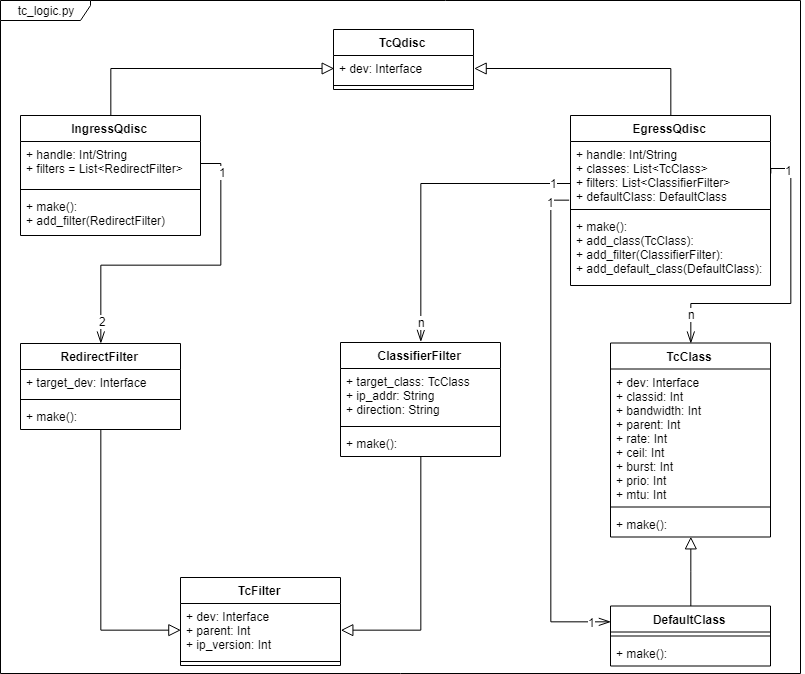
\includegraphics[width=\textwidth]{img/tc_logic_uml.png}
    \caption{UML-Model of \text{tc\_logic.py}}
    \label{tc_logic_uml}
\end{figure}
